\chapter{Virtualization}
\label{chap:virtualnetworks}
\emph{In this chapter, (the) three types of virtualization will be explained in detail: machine virtualization, network virtualization and storage virtualization.}

Before digging deeper into security aspects in virtual networks, some types of virtualization must first be defined.
\section{Machine virtualization - Hypervisors}
In order to be able to run virtual machines, a hypervisor is needed. Chapter \ref{chap:introduction} already described the function of a hypervisor, also called a virtual machine manager \citep{Techtarget}: a hypervisor abstracts the physical resources - CPU, memory, disks, network adapters, \ldots - from systems running on top of it. So it allows for a physical machine (that we will call a host) to share their hardware resources amongst virtual machines (that we will call guests) running as guests on top of the host (the physical hardware). Note that a hypervisor is nothing more than a piece of software \citep{Datacenter} that ensures that VM's do not interrupt each other \citep{Techtarget}.

Each VM appears to have it's own processor, memory and disk. However, the hypervisor is actually controlling the VM's resources and allocating the resources to their needs \citep{Techtarget}. 

There exist two types of hypervisors:  \textbf{Type 1} and \textbf{Type 2} hypervisors \citep{Techtarget2}. Type 1 hypervisors are the so-called \textbf{Bare-metal hypervisors} whereas type 2 hypervisors are known as \textbf{hosted hypervisors}. Both will be discussed in the upcoming sections.

From know on, the physical machine will be called the \textbf{host} and the virtual machine that runs on top of the host (through the hypervisor), will be called the \textbf{guest}.

\subsection{Bare-metal hypervisors}
\label{sec:baremetal}
The name `bare-metal' (``without an operating system'') comes from the fact that this type of hypervisor is deployed as a bare-metal installation. This implies that it is not required to first install a server operating system: the hypervisor is the first thing to be installed on the host \citep{Techtarget2}. To be precise: the hypervisor is installed as the operating system of the host \citep{Datacenter}.

A bare-metal hypervisor runs directly on the host's hardware and therefore allow for direct access to the hardware recourses, which results in greater performance compared to hosted hypervisors \citep{Techtarget2} as illustrated in the picture below. One point of remark: the VM's running on top of the hypervisor do not have direct access to the hardware recourses. Instead, they have a virtual view of for example the processor and run in a private memory address region that is unique for each guest \citep{HyperVArch}. Only the hypervisor has direct access to the hardware.

\begin{figure}[h]
    \centering
    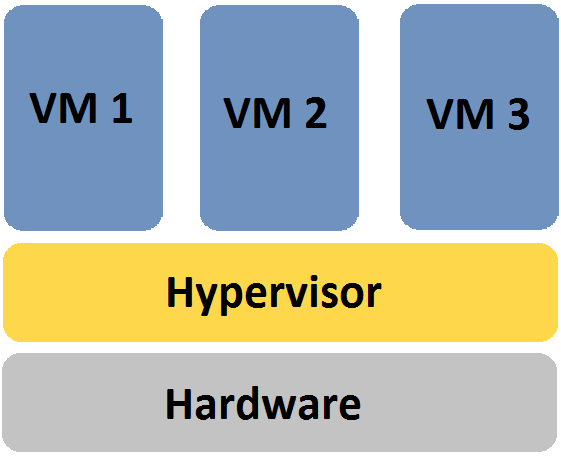
\includegraphics[width=0.55\textwidth]{BareMetal.png}
    \caption[Bare-metal hypervisor]{A schematic architecture of a typical bare-metal hyervisor. As one can see, the hypervisor runs directly on the host's hardware and therefore has direct access to the hardware.}
\end{figure}

\subsubsection{Hyper-V}

Hyper-V is a bare-metal hypervisor developed by Microsoft \citep{HyperV}. Hyper-V is the replacor of Microsoft Virtual PC in newer versions of Windows\citep{HyperVSuccessor} and was first included in Windows Server 2008, where system administrators could enable the Hyper-V role \citep{HyperV2}. Hyper-V only supports x64 versions of Windows Server 2008 and Windows Server 2012 \citep{HyperVArch}.

The Hyper-V role provides the software infrastructure and management tools to create and manage a virtualized computer environment. As previously explained in section \ref{sec:securityRegardingVirtualization}, each VM runs in a isolated computing environment \citep{HyperVOverview}. In Hyper-V, this isolation is achieved by means of partitions \citep{HyperVArch}.

\paragraph{Architecture of Hyper-V}

In order for Hyper-V to work, a root partition (also known as parent partition) must be present on top of the hypervisor running a 64 bit version of Windows Server 2008 or Windows Server 2012. \citep{HyperVArch}. It also runs the virtualization stack, contains the device drivers and therefore has direct access to the hardware resources as well \citep{HyperVArch2}.

In essential, this root partition is nothing more than a virtual machine running Windows Server 2008 or Windows Server 2012 used to control the other guest VM's. The machine that installed the Hyper-V role, becomes the root partition.
The root partition can be compared to the Dom0 VM of the Xen Project hypervisor explained in section \ref{subsub:Xen}. \\ \\
The picture below visualizes the Hyper-V's architecture.
\begin{figure}[h]
    \centering
    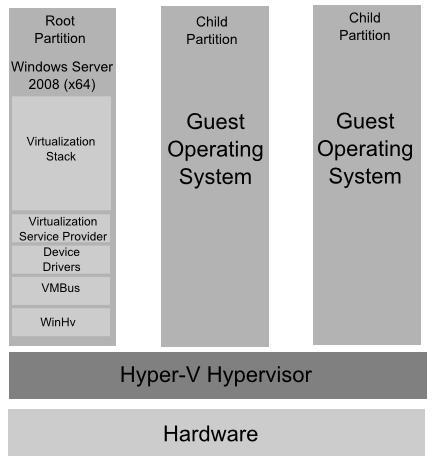
\includegraphics[width=0.55\textwidth]{HyperVArch.jpg}
    \caption[Hyper-V Architecture]{The architecture of the Hyper-V hypervisor. The root partion contains the Virtualization Stack which, in his turn, contains a collection of tools that provide the Hyper-V functionality, for example the virtual devices and the device drivers.}
\end{figure}

%\paragraph{Scheduling in Hyper-V}

\clearpage

\subsubsection{Xen}
\label{subsub:Xen}
The Xen Project hypervisor is the only open source bare-metal hypervisor available at the time of writing. It consists of four main components being the Xen Project hypervisor, the guest VM's, the Control Domain and the Toolstack \citep{Xen1}. \\
\paragraph{Architecture of the Xen Project hypervisor}
The Xen hypervisor runs directly on the hardware and contains the scheduler. It is responsible for handling interrupts, CPU time and memory usage. The hypervisor is the first program to run after exiting the bootloader \citep{Xen1}.\\ \\
The Control Domain (Dom0) is a special type of virtual machine. Compared to the other guest VM's, this Dom0 has special privileges. E.g.: it is able to access the hardware directly and interacts with the other VM's. Therefore, the Dom0 contains the drivers for the hardware and a toolstack \citep{Xen1}.

One could compare this Dom0 with the root partition of Hyper-V.

The Dom0 is the first VM to be started by the hypervisor.\\ \\
The Toolstack (xl is the prefered toolstack at the time of writing \citep{Xen2}) allows users to manage their VM's \citep{Xen1}.\\ \\
The guest VM's run on top of the Xen hypervisor and run their own operating system and application software. These are the actual VM's. \\
The picture below visualizes the Xen Project hypervisor's architecture \citep{Xen2}.
\begin{figure}[h]
    \centering
    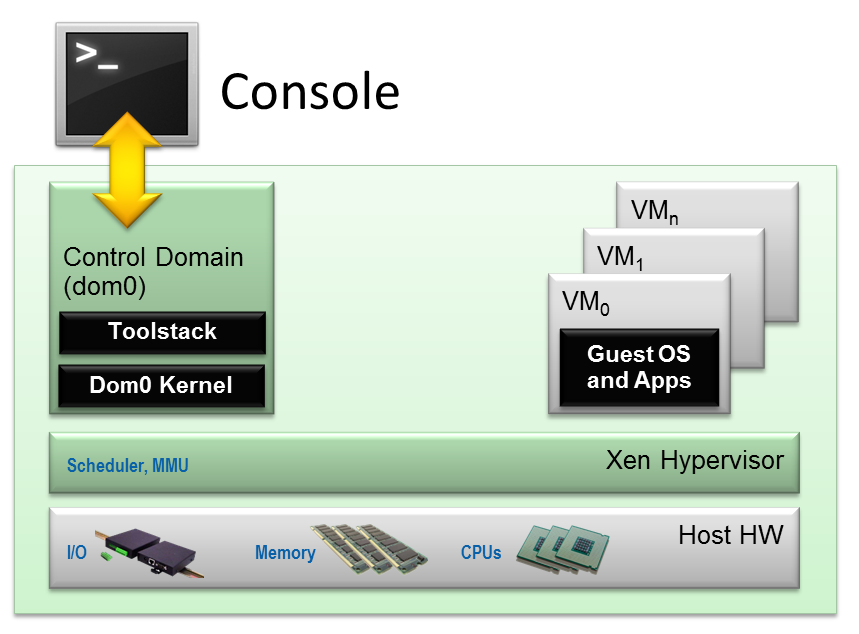
\includegraphics[width=0.45\textwidth]{Xen_Arch_Diagram.png}
    \caption[Xen architecture]{The architecture of the Xen Project hypervisor. It consists of four main components: the hypervisor itself, the guest VM's, the Control Domain and the Toolstack for managing the VM's.}
\end{figure}

\clearpage

\subsubsection{VMware ESXi}

VMware ESXi the bare-metal hypervisor developed by VMware. It is the successor of the ESX hypervisor \citep{VMware1}.

\paragraph{Architecture of the ESXi hypervisor}

The VMware ESXi hypervisor consists of the VMkernel, which is the underlying operating system and processes that run on top of the VMkernel.

The VMkernel contains the drivers, the management agents and applications and hardware monitoring components. The processes run on top of it are the Direct Console User Interface (DCUI), the virtual machine monitor (VMM) together with the helper processes VMX. Each VM has its own VMM and VMX process.
On top of the VMkernel run the guest VM's. \\ \\
The DCUI is responsible for low-level configuration and management. It is accessible through the server console and is used for basic, initial configuration.

The VMM is a process that provides an execution environment for the virtual machines, together with some helper processes knows as VMX processes.

Note that - in contrast to Hyper-V and Xen, there does not exist a fully functional console OS that manages the VM's. Instead, only a small POSIX kernel is included. This implies that the footprint of the hypervisor is very small - not more than 32MB.

\begin{figure}[h]
    \centering
    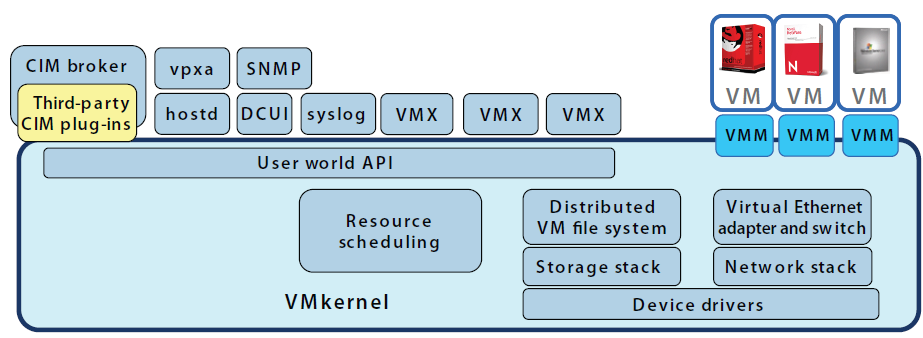
\includegraphics[width=0.65\textwidth]{VMware1.png}
    \caption[VMware architecture]{...}
\end{figure}
 \clearpage
\begin{figure}[h]
    \centering
    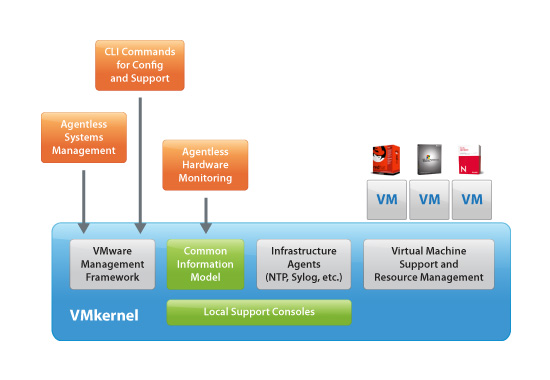
\includegraphics[width=0.55\textwidth]{VMware2.jpg}
    \caption[VMware simplified architecture]{...}
\end{figure}


The architectures of these 3 hypervisors are roughly equal \ldots .
In this thesis, Hyper-V will be used.
\subsection{Hosted hypervisors}

As described in section \ref{sec:baremetal}, bare-metal hypervisors run directly on top of the hardware. However, another type of hypervisor exist that runs on top of an existing operating system: the hosted hypervisors or type-2 hypervisors.

So basically, this means that an operating system is installed inside another operating system in contrast to the bare-metal hypervisor where each OS has direct access (through the hypervisor) to the hardware.

An example of such a hosted hypervisor is VirtualBox \citep{VirtualBox}.

\section{Network virtualization}

After having defined virtual machines and the hypervisors, it is now time to focus how a virtual machine is able to communicate with the outside world and to have a closer look how internal (i.e.: inside the hypervisor) network virtualization works. \\ \\
When one wants to provide a VM with network capabilities, at lease one virtual network interface card (vNIC) has to be assigned to this VM - just as a physical computer requires a physical NIC as well  \citep{Technet1}.

As Hyper-V will be used in this thesis, the focus of internal virtual networking will be stressed on Hyper-V. \\ \\

One must not forget that a virtual network is actually just a software logic that is part of Hyper-V and sents and receives packets in OSI layer 2. \\

There exist three different types of virtual networks in Hyper-V: external virtual networks, internal virtual networks and private virtual networks \citep{HyperVNetworking2}. Each of them will be explained in the following section.

\subsection{External virtual network}

Virtualization is all about abstracting existing hardware as explained in the first chapter. The same concept is used for virtual networking. Consider a host with an arbitrary number of cores and an arbitrary amount of RAM which hosts 50 VM's, but with only one physical NIC.

The requests performed by the virtual NIC's of the VM's can overhelm the physical NIC of the host. To overcome this problem, Microsoft developed an abstraction layer that uses the Virtual Switch concept \citep{HyperVNetworking1}.

This abstraction layer sits in between the the physical NIC and the vNIC's of the different VM's. It therefore abstracts the physical NIC. Microsoft calls this \emph{External Networking} \citep{HyperVNetworking2} and is illustrated in the figure below \citep{HyperVNetworking1}.\\
\begin{figure}[h]
    \centering
    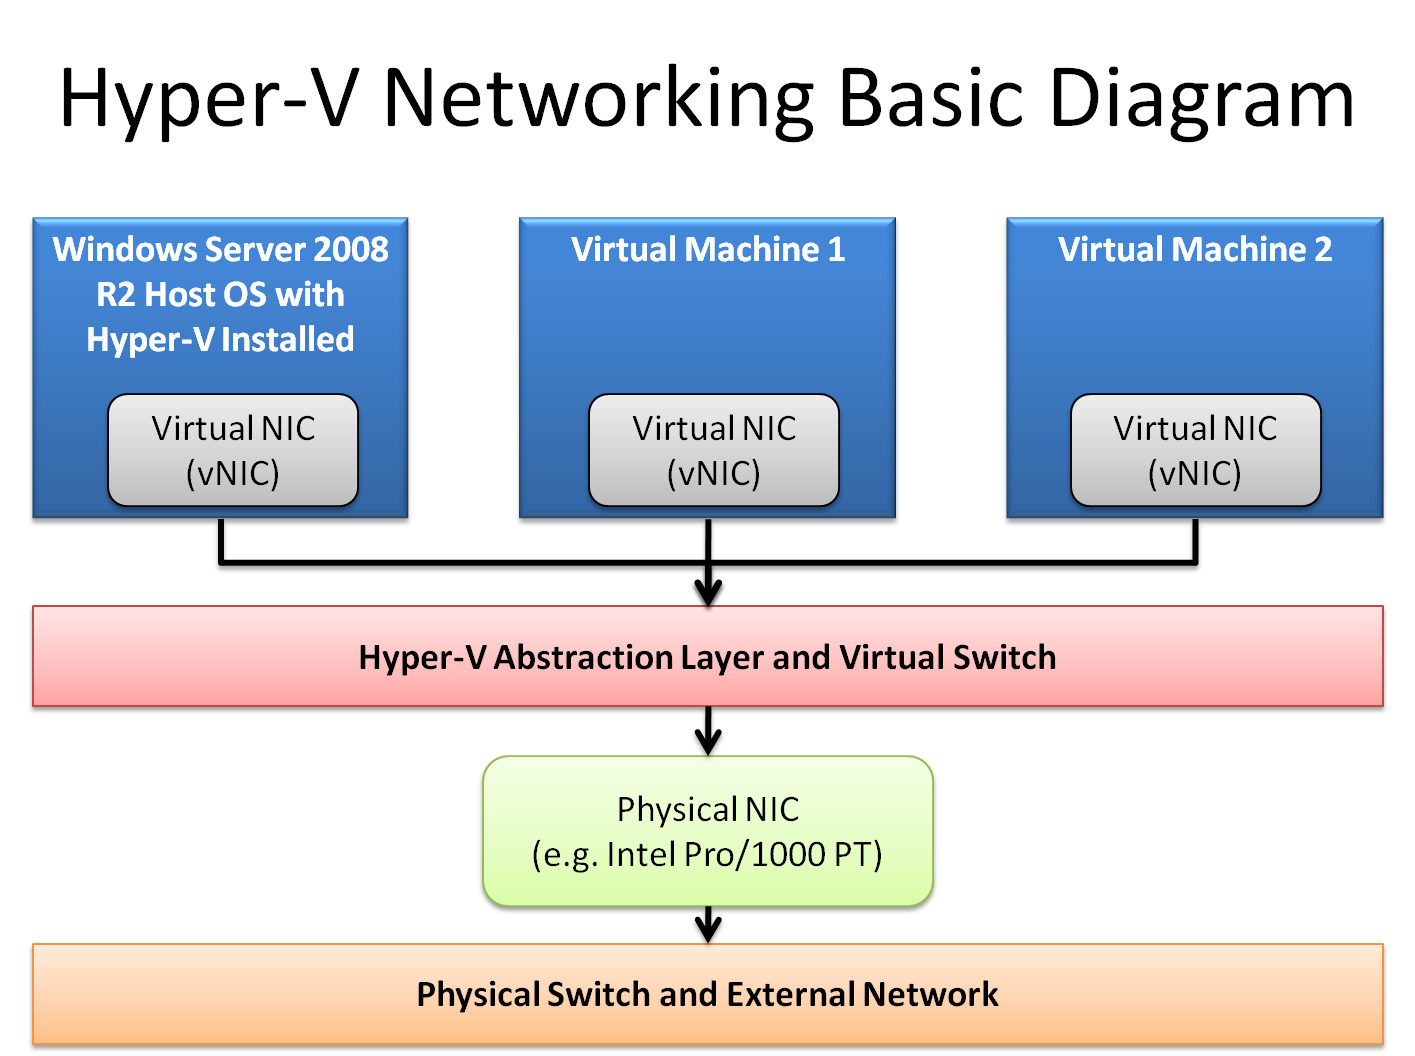
\includegraphics[width=0.65\textwidth]{ExternalNetwork.png}
    \caption[Microsoft Virtual Switch concept]{The concept of virtual networking as an abstraction layer on top of the physical NIC. The purple layer represents the virtual switch. Note that this is only occurs with external networking - internal and private networking do not use virtual switches.}
\end{figure}
When creating an external virtual network in Hyper-V, the following changes take place:
\begin{itemize}
\item The host creates a new virtual NIC that is used to connect to the physical network. So a minimum of two network adapters exist on the host.
\item The Microsoft Virtual Switch Protocol is bound to the physical NIC.
\end{itemize}
Once created, the virtual network will work exactly the same as a phyiscal network, with that difference that the switch is a software-matic; additional ports (NICs) can be added dynamically.
Following figure visualizes the external network concept of Hyper-V.
\begin{figure}[h]
    \centering
    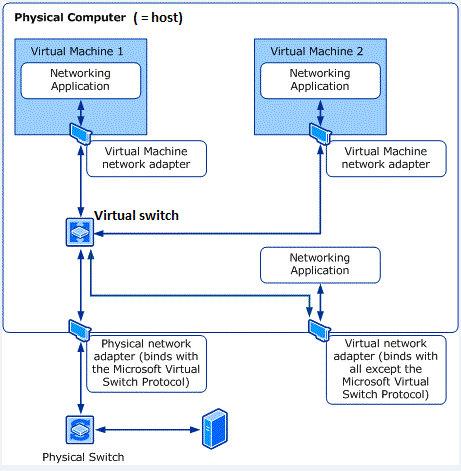
\includegraphics[width=0.65\textwidth]{ExternalNetwork_2.png}
    \caption[External Virtual Network]{A diagram of the different components of external networking. The physical NIC binds with the virtual switch. The networking applications of the host communicate with the external network (the physical switch) through the newly created virtual NIC. Note that each VM is assigned a virtual NIC.}
\end{figure}
The external network type has the following capabilities \citep{HyperVNetworking3}:
\begin{itemize}
\item It allows for communication between a VM and and an external network so that all VM's are visible as seperate hosts on the external network  as if they would be dedicated, physical hosts. One can compare this with Xen bridged networking \citep{XenNetworking}.
\item It allows for communication between VM's on the same host.
\item It allows for communication between the VM's and the host.
\end{itemize}

\subsection{Internal virtual network}

In an internal virtual network, the phyiscal adapter plays no role in the network and is therefore not bounded. Thus access and communication to external networks (including the LAN outside the virtual machine) is impossible \citep{HyperVNetworking1, HyperVNetworking3}. However, communication with the host is possible. \\
Some characteristics of internal networks are \citep{HyperVNetworking2}:
\begin{itemize}
\item It allows for communication between VM's on the same host.
\item It allows for communication between VM's and the host.
\end{itemize}
The figure below visualizes this concept \citep{HyperVNetworking2}:
\begin{figure}[h]
    \centering
    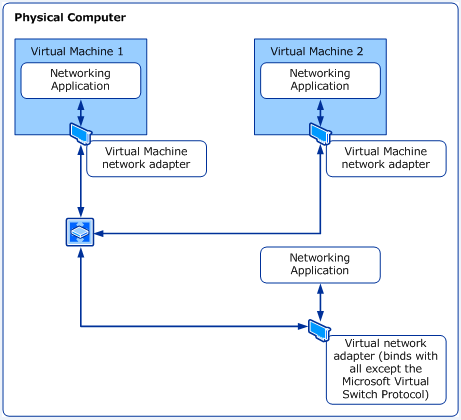
\includegraphics[width=0.65\textwidth]{InternalNetwork.png}
    \caption[Internal Virtual Network]{...}
\end{figure}

\subsection{Private virtual network}

When a private virtual network is used, VM's are only able to communicate with each other. No communication with the host exist, however. That is the difference with an internal private network. \\
Some characteristics of internal networks are \citep{HyperVNetworking2}:
\begin{itemize}
\item Communication between VM's only.
\end{itemize}
he figure below visualizes this concept \citep{HyperVNetworking2}:
\begin{figure}[h]
    \centering
    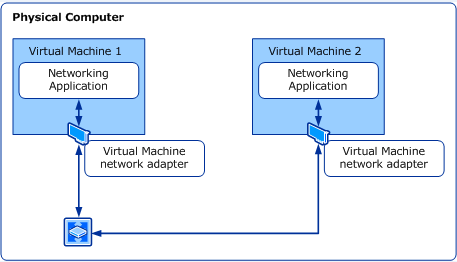
\includegraphics[width=0.65\textwidth]{PrivateNetwork.png}
    \caption[Private Virtual Network]{...}
\end{figure}

\subsection{External network virtualization}

VLAN's, \ldots . Moet aan de prof vragen of dit ook moet.

\clearpage

\section{Storage virtualization}

\subsection{Host-based storage virtualization}

Host-based storage virtualization adds, as any virtualization technique (see chapter \ref{chap:introduction}), a layer of abstraction between the host OS and the physical disks. Each mayor OS provides a piece of software called a logical volume manager to provide such a layer of abstraction \citep{VHD3}. \\
Whereas in traditional disk management, the OS looks for physical disks and partitions that reside on those physical disks, with a logical volume manager disks can be abstracted. This way, a logical disk can span multiple physical disk and appear in the OS as one disk.

A logical volume manager adds more flexibility in a way that logical volumes can be resized and moved around. This is not a straightforward job when physical disks and partitions are used \citep{VHD2}. \\
Microsoft's implementation of logical volume management is called Logical Disk Manager. In the next section, virtual hard disks in Hyper-V will be discussed. \\
The next figure illustrates the concept of Logical Volume Management.
\begin{figure}[h]
    \centering
    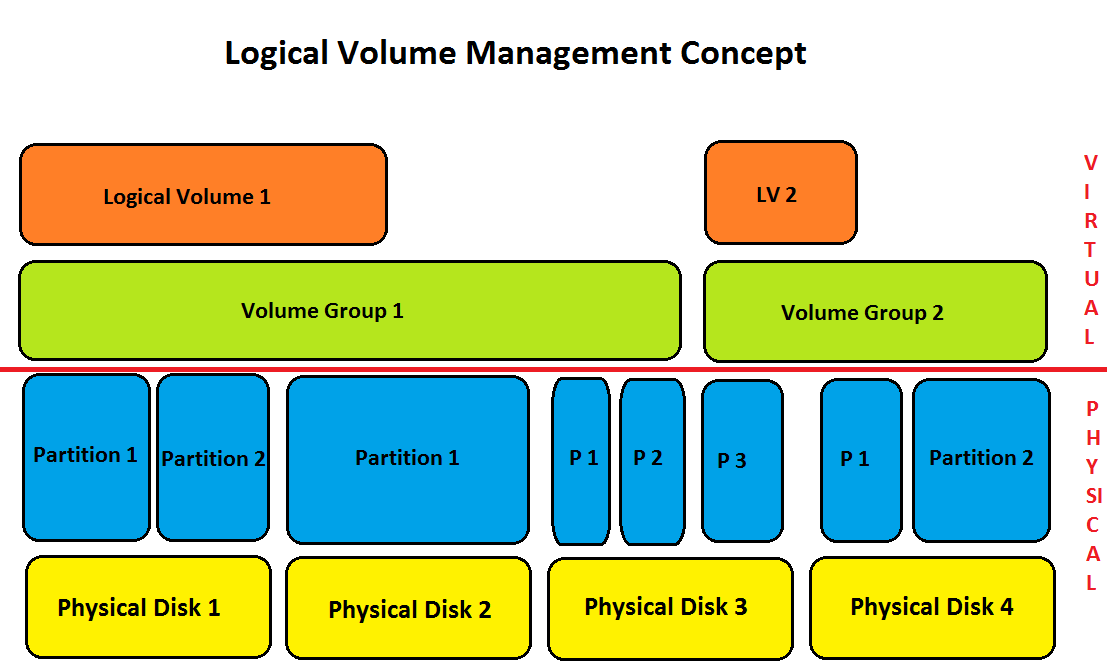
\includegraphics[width=0.85\textwidth]{LVM.png}
    \caption[Logical Volume Management]{LVM adds a layer of abstraction between the OS and the phyical disks / partitions. In the figure, a volume group spans 5 physical partitions and disks. On top of the volume group lies a logical volume (partition). As one can see, there is space left on the volume group and thus expanding the logical volume (partition) is possible. With a phyiscal partition, this would not be possible without losing data.}
\end{figure}
\subsection{Virtual hard disks in Hyper-V}

A virtual hard disk (with extension .vhd) enables one to create a virtual disk which resides on the physical disk as a single file \citep{VHD1}.
A VHD has the same capabilities as a physical disk and thus are used the same way. They are able to host file systems and support standard disk operations \citep{VHD1}.